The goal was to achieve a muscle activation driven pointing task using a 2-DoF, 6-muscle arm model. 
In addition to muscle-induced torques, pure joint torques could compensate for the model weaknesses.
The first three Lagrange terms of the objective function (Eq.~\ref{eq:cost_pointing}) were added for control regularization (muscle activation $a$ and joint torques $\tau$) and for state ($x$) regularization.
The last Mayer term corresponds to the pointing tasks at the final node, to superimpose two markers, the first one, $m_u$, fixed in the ulna system of coordinates and the second one, $m^*_s$, fixed in the scene.
:

\[
\begin{aligned}
	\mathcal{C} = &\int_{t=0}^T\underbrace{\|a\|^2}_{\mathtt{MIN\_ACTIVATION}}~
	+\underbrace{\|\tau\|^2}_{\mathtt{MIN\_TORQUE}}~
	+\underbrace{\|x\|^2}_{\mathtt{MIN\_STATE}}~ dt,\\
	&+ \omega_1~\underbrace{\|m_u-m^*_s\|^2}_{\mathtt{TRACK\_MARKERS}}~
\end{aligned}
\addtag
\label{eq:cost_pointing}
\]
%

\noindent where T is the duration of the motion, and $\omega_1=1e5$.
The movement lasted for 2~seconds and was discretized using 50 shooting nodes.
The problem was solved using IPOPT and ACADOS resulting in two significantly different solutions.
ACADOS provided a 16 times smaller optimized cost (Tab.~\ref{tab:Perfs_and_detailed_implementations_of_each_example}), which illustrate the pitfalls of local minima as well as the benefits of having straightforward access to different solvers.  
Indeed, the ACADOS-based solution (Fig.~\ref{fig:snapshots_activation_driven_pointing}, top) makes good use of gravity to minimize the control inputs, while the IPOPT-based solution (Fig.~\ref{fig:snapshots_activation_driven_pointing}, bottom) moved the arm in the opposite direction and was stuck in a local minimum (still achieving the task though). 
It is worth mentioning that for the purpose of this illustration, no constraint was given about the shoulder range of motion to ensure physiological muscle trajectories. 

 
 

%
\begin{figure*}[t!]
\centering
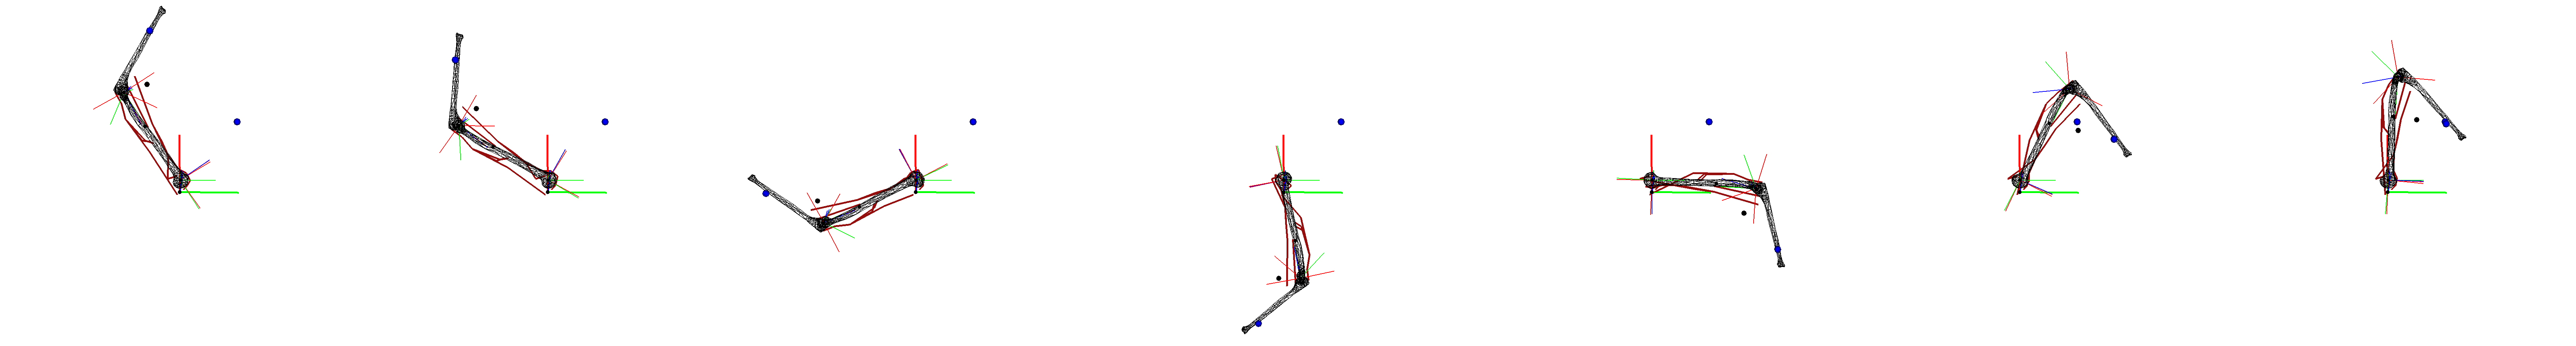
\includegraphics[width=\textwidth]{figures/activation_pointing_snapshots_acados.png}\\
\vspace*{0.5em}
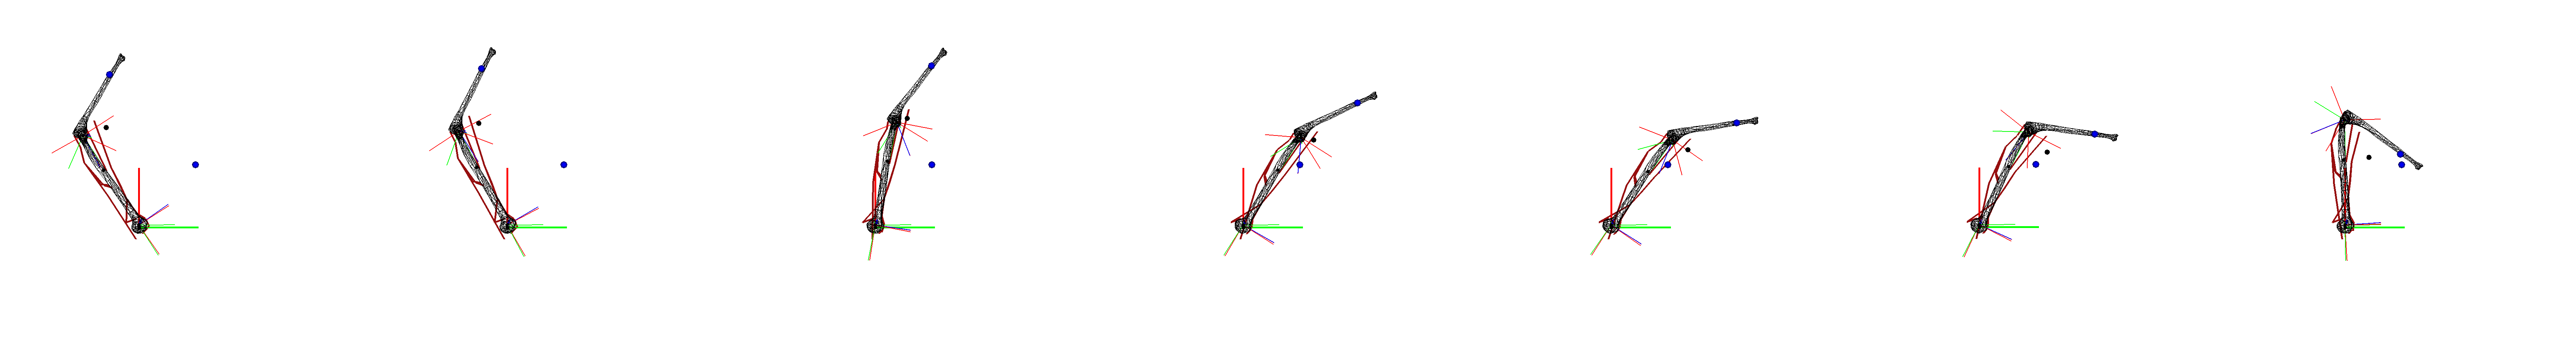
\includegraphics[width=\textwidth]{figures/activation_pointing_snapshots_ipopt.png}
\caption{Snapshots of an optimized muscle activation driven pointing task. Top: using ACADOS. Bottom: using IPOPT.}
\label{fig:snapshots_activation_driven_pointing}
\end{figure*}
%









